
\chapter{Iteration}
\label{iteration}

This chapter is about iteration, which is the ability to run
a block of statements repeatedly.  We saw a kind of iteration,
using recursion, in Section~\ref{recursion}.
We saw another kind, using a {\tt for} loop,
in Section~\ref{for_loops}.  In this chapter we'll see yet another
kind, using a {\tt while} statement.
But first we want to say a little more about variable assignment.

\section{Assignment Versus Equality}
\index{assignment!operator}
\index{equality operator}

Before going further, I want to address a common source of confusion.
Because Perl uses the equals sign ({\tt =}) for assignment, it is
tempting to interpret a statement like {\tt \$a = \$b} as a
mathematical proposition of equality, that is, the claim that 
{\tt \$a} and {\tt \$b} are equal.  But this interpretation is 
wrong.
\index{equality and assignment}

First, equality is a symmetric relationship and assignment is not.  For
example, in mathematics, if $a=7$ then $7=a$.  But in Perl, the
statement {\tt \$a = 7} is legal and {\tt 7 = \$a} is not.

Also, in mathematics, a proposition of equality is either true or
false for all time.  If $a=b$ now, then $a$ will always equal $b$.
In Perl, an assignment statement can make two variables equal, but
they don't have to stay that way:

\begin{verbatim}
> my $a = 5;
5
> my $b = $a;   # $a and $b are now equal
5
> $a = 3;       # $a and $b are no longer equal
3
> say $b;
5
\end{verbatim}
%
The third line changes the value of {\tt \$a} but does not 
change the value of {\tt \$b}, so they are no longer equal. 

In brief, remember that {\tt =} is an assignment operator and  
not an equality operator; the operators for testing equality 
between two terms are {\tt ==} for numbers and {\tt eq} for strings.

\section{Reassignment}
\index{assignment}
\index{statement!assignment}
\index{reassignment}

As you may have discovered, it is legal to make more than one
assignment to the same variable.  A new assignment makes an existing
variable refer to a new value (and stop referring to the old value):

\begin{verbatim}
> my $x = 5;
5
> say $x;
5
> $x = 7;
7
> say $x
7
\end{verbatim}
%
The first time we display 
{\tt \$x}, its value is 5; the second time, its
value is 7.

Figure~\ref{fig.assign2} shows what {\bf reassignment} looks
like in a state diagram. \index{state diagram} \index{diagram!state}

Reassigning variables is often useful, but you should use this feature 
with some caution.  If the values of variables change frequently, it can
make the code difficult to read and debug.

\begin{figure}
\centerline
{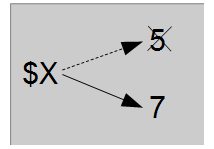
\includegraphics[scale=0.5]{figs/reassignment.png}}
\caption{State diagram.}
\label{fig.assign2}
\end{figure}



\section{Updating Variables}
\label{update}

\index{update}
\index{variable!updating}

A common kind of reassignment is an {\bf update},
where the new value of the variable depends on the old:

\begin{verbatim}
> $x = $x + 1;
\end{verbatim}
%
This means ``get the current value of {\tt \$x}, add one, and then
update {\tt \$x} with the new value.''

If you try to update a variable that has not been given a value, 
you get a warning, because Perl evaluates the right side 
of the assignment statement before it assigns a value to {\tt \$x}:

\begin{verbatim}
> my $x;
> $x = $x + 1;
Use of uninitialized value of type Any in numeric context 
 in block <unit> at <unknown file> line 1
\end{verbatim}
%
Before you can update a variable, you have to declare it and 
{\bf initialize} it, usually with an assignment statement:
\index{initialization (before update)}

\begin{verbatim}
> my $x = 0;
> $x = $x + 1;
\end{verbatim}
%
Updating a variable by adding 1 is called an {\bf increment};
subtracting 1 is called a {\bf decrement}.
\index{increment operator}
\index{decrement operator}

As mentioned earlier in Section~\ref{expr_and_statements}, 
Perl has some shortcuts for increment and decrement :

\begin{verbatim}
$x += 1; # equivalent to $x = $x + 1
$x++;    # also equivalent 

$x -= 1; # equivalent to $x = $x - 1
$x--;    # also equivalent 
\end{verbatim}

\section{The {\tt while} Statement}
\index{statement!while}
\index{while loop}
\index{loop!while}
\index{iteration}

Computers are often used to automate repetitive tasks.  Repeating
identical or similar tasks without making errors is something that
computers do well and people do poorly.  In a computer program,
repetition is also called {\bf iteration}.

We have already seen two functions, {\tt countdown} and
\verb"print-n-times", that iterate using recursion 
(see Section~\ref{recursion}).  Because 
iteration is so common, most programming languages including 
Perl provide language features to make it easier.
One is the {\tt for} statement we saw in Section~\ref{for_loops}.
We'll get back to that later.

Another is the {\tt while} statement.  Here is a version of {\tt
countdown} that uses a {\tt while} statement:

\begin{verbatim}
sub countdown(Int $n is copy) {
    while $n > 0 {
        say $n;
        $n--;
    }
    say 'Blastoff!';
}
\end{verbatim}
%
You can almost read the {\tt while} statement as if it were English.
It means, ``While {\tt \$n} is greater than 0,
display the value of {\tt n} and then decrement
{\tt \$n}.  When you get to 0, display the word {\tt Blastoff!}''
\index{flow of execution}

More formally, here is the flow of execution for a {\tt while} statement:

\begin{enumerate}

\item Determine whether the condition is true or false.

\item If false, exit the {\tt while} statement
and continue execution at the next statement.

\item If the condition is true, run the
body and then go back to step 1.

\end{enumerate}

This type of flow is called a loop because the third step
loops back around to the top.  
\index{condition}
\index{loop}
\index{body}

The body of the loop should change the value of one or more variables
so that the condition becomes false eventually and the loop
terminates.  Otherwise, the loop will repeat forever, which is called
an {\bf infinite loop}.  An endless source of amusement for computer
scientists is the observation that the directions on shampoo,
``Lather, rinse, repeat,'' are an infinite loop.
\index{infinite loop}
\index{loop!infinite}

In the case of {\tt countdown}, we can prove that the loop
terminates: if {\tt \$n} is zero or negative, the loop never runs.
Otherwise, {\tt \$n} gets smaller each time through the
loop, so eventually we have to get to 0.

For some other loops, it is not so easy to tell whether the 
loop terminates.  For example:

\begin{verbatim}
sub sequence($n is copy) {
    while $n != 1 {
        say $n;
        if $n %% 2 {        # $n is even
            $n = $n / 2;
        } else {            # $n is odd
            $n = $n*3 + 1
        }
    }
    return $n;
}
\end{verbatim}
%
The condition for this loop is {\tt \$n != 1}, so the loop will continue
until {\tt \$n} is {\tt 1}, which makes the condition false.

Each time through the loop, the program outputs the value of {\tt \$n}
and then checks whether it is even or odd.  If it is even, {\tt \$n} is
divided by 2.  If it is odd, the value of {\tt \$n} is replaced with
{\tt \$n*3 + 1}. For example, if the argument passed to {\tt sequence}
is 42, the resulting values of {\tt n} are 42, 21, 64, 32, 16, 8, 4, 2, 1.

Since {\tt \$n} sometimes increases and sometimes decreases, there is no
obvious proof that {\tt \$n} will ever reach 1, or that the program
terminates.  For some particular values of {\tt n}, we can prove
termination.  For example, if the starting value is a power of two,
{\tt n} will be even every time through the loop
until it reaches 1. The previous example ends with such a sequence
of powers of two, starting with 64.
\index{Collatz conjecture}

The hard question is whether we can prove that this program terminates
for {\em all} positive values of {\tt n}.  So far, no one has
been able to prove it {\em or} disprove it!  (See
\url{http://en.wikipedia.org/wiki/Collatz_conjecture}.)

As an exercise, you might want to rewrite the function 
\verb"print-n-times" from Section~\ref{recursion} using 
iteration instead of recursion.

\index{statement modifier}
\index{postfix!syntax}
The {\tt while} statement can also be used as a statement modifier (or postfix syntax):

\begin{verbatim}
my $val = 5;
print "$val " while $val-- > 0;   # prints 4 3 2 1 0
print "\n";
\end{verbatim}

The {\tt while} loop statement executes the block as long as 
its condition is true. There is also an {\tt until} loop 
statement, which executes the block as long as its condition 
is false:
\index{until loop}

\begin{verbatim}
my $val = 1;
until $val > 5 {
    print $val++;                 # prints 12345
}
print "\n";
\end{verbatim}

\section{Local Variables and Variable Scoping}

We have seen in Section~\ref{localvar} that variables created 
within a subroutine (with the {\tt my} keyword) are \emph{local} 
to that subroutine. The {\tt my} 
keyword is often called a \emph{declarator}, because it 
is used for declaring a new variable (or other identifier). 
It is by far the most common declarator. Other declarators 
include {\tt our} or {\tt state}, briefly described later 
in this chapter. 
\index{lexical scope}
\index{lexical variable}
\index{variable!lexical}
\index{my}
\index{declarator}

Similarly, subroutine 
parameters are also usually \emph{local} to the subroutine 
in the signature of which they are declared.
\index{subroutine parameters}

We briefly mentioned that the term \emph{lexically scoped} 
is probably more accurate than local, but it was 
too early at that point to really explain what this means.

Declaring a variable with {\tt my} gives it \emph{lexical 
scope}. This means it only exists within the current block. 
Loosely speaking, a 
block is a piece of Perl code within curly brackets or 
braces. For example, the body of a subroutine and the code of a 
{\tt while} or {\tt for} loop or of an {\tt if} conditional
statement are code blocks. Any variable created with the 
{\tt my} declarator exists and is available for use only 
between the place where it is declared and the end of the 
enclosing code block.
\index{bracket!curly}
\index{curly bracket}

For example, this code:

\begin{verbatim}
if $condition eq True {
    my $foo = "bar";
    say $foo;  # prints "bar"
}
say $foo;      # ERROR: "Variable '$foo' is not declared ..."
\end{verbatim}
%
will fail on the second print statement, because the \verb'say' 
function call is not in 
the lexical scope of the {\tt \$foo} variable, which ends 
with the closing brace of the condition block. If we want 
this variable to be accessible after the end of the condition, 
then we would need to declare it before the {\tt if} statement. 
For example:

\begin{verbatim}
my $foo;
if $condition eq True {
    $foo = "bar";
    say $foo;  # prints "bar"
} else {
    $foo = "baz";
}
say $foo;      # prints "bar" or "baz" depending on $condition
\end{verbatim}
%
If a lexical variable is not declared within a block, its 
scope will extend until the end of the file (this is sometimes 
called a static or a global variable, although these terms are 
somewhat inaccurate). For example, in the last code snippet 
above, the scope of the {\tt \$foo} variable will extend 
until the end of the file, which may or may not be a good thing, 
depending on how you intend to use it. It 
is often better to reduce the scope of variables as much as 
possible, because this helps reduce dependencies between 
various parts of the code and limits 
the risk of subtle bugs. In the code above, if we want to 
limit the scope of {\tt \$foo}, we could add braces to create 
an enclosing block for the sole purpose of limiting the scope:
\begin{verbatim}
{
    my $foo;
    if $condition eq True {
        $foo = "bar";
        say $foo;  # prints "bar"
    } else {
        $foo = "baz";
    }
    say $foo;      # prints "bar" or "baz" depending on $condition
}
\end{verbatim}
% 
Now, the outer braces create an enclosing block limiting the 
scope of {\tt \$foo} to where we need it. This may seem to be a 
somewhat contrived example, but it is not uncommon to add 
braces only for the purpose of precisely defining the scope 
of something.

Lexical scoping also means that variables with the same names
can be temporarily redefined in a new scope: 

\begin{verbatim}
my $location = "outside";
sub outer {
    say $location;
}
sub inner {
    my $location = "inside";
    say $location;
}
say $location;   # -> outside
outer();         # -> outside
inner();         # -> inside
say $location;   # -> outside
\end{verbatim}
% 
We have in effect two variables with the same name, 
{\tt \$location}, but different scopes. One is valid only 
within the {\tt inner} subroutine where it has been redefined, 
and the other anywhere else.

If we add a new subroutine:
\begin{verbatim}
sub nowhere {
    my $location = "nowhere";
    outer();
}
nowhere();       # -> outside
\end{verbatim}
% 
this will still print ``outside,'' because the {\tt outer} 
subroutine knows about the ``outside'' version of the 
{\tt \$location} variable, which existed when {\tt outer} was defined.
In other word, the {\tt outer} code that referenced to the 
outer variable (``outside'') knows about the variable that existed 
when it was created, but not about the variable existing where 
it was called. This is how \emph{lexical} variables work. 
This behavior is the basis for building \emph{closures}, a  
form of subroutine with some special properties that we 
will study later in this book, but 
is in fact implicitly present everywhere in Perl~6.
\index{closure}
\index{variable!lexical}
\index{lexical variable}

While having different variables with the same name can give 
you a lot of expressive power, we would 
advise you to avoid creating different variables with the 
same name and different scopes, at least until you really understand 
these concepts well enough to know what you are doing, as this 
can be quite tricky.

By far, most variables used in Perl are lexical variables, 
declared with the {\tt my} declarator. Although they are 
not declared with {\tt my}, parameters declared 
in the signature of subroutines and parameters of pointy 
blocks also have a lexical scope limited to the body of the 
subroutine or the code block.
\index{my}
\index{declarator}

There are other declarators, such as {\tt our}, which creates 
a package-scoped variable, and {\tt state}, which creates a 
lexically scoped variable but with a persistent value. They 
are relatively rarely used.
\index{our}
\index{state}

One last point: although they are usually not declared with 
a {\tt my} declarator, subroutines themselves also have by default
a lexical scope. If they are defined within a block, they will 
be seen only within that block. An example of this has been 
given at the end of the solution to the GCD exercise of the 
previous chapter (see Subsection~\ref{sol_gcd}). 
That being said, you \emph{can} declare a subroutine 
with a {\tt my} declarator if you wish:

\begin{verbatim}
my sub frobnicate { 
    # ... 
}
\end{verbatim}

This technique might add some consistency or some form of 
self-documenting feature, but you won't buy very much 
added functionality with that.
 

\section{Control Flow Statements ({\tt last}, {\tt next}, etc.)}
\index{control flow}
\index{flow!control}
\index{last statement}
\index{statement!last}
\index{next statement}
\index{statement!next}

Sometimes you don't know it's time to end a loop until you get half
way through the body.  In that case, you can use a control flow 
statement such as {\tt last} to jump out of the loop.

For example, suppose you want to take input from the user until they
type {\tt done}.  You could write:

\begin{verbatim}
while True {
    my $line = prompt "Enter something ('done' for exiting)\n";
    last if $line eq "done";
    say $line;
}
say 'Done!';
\end{verbatim}
%
The loop condition is {\tt True}, which is always true, so the
loop runs until it hits the {\tt last} statement.

Each time through, it prompts the user to type something.
If the user types {\tt done}, the {\tt last} statement exits
the loop.  Otherwise, the program echoes whatever the user types
and goes back to the top of the loop.  Here's a sample run:

\begin{verbatim}
$ perl6 while_done.pl6
Enter something ('done' for exiting)
Not done
Not done
Enter something ('done' for exiting)
done
Done!
\end{verbatim}
%
This way of writing {\tt while} loops is common because you
can check the condition anywhere in the loop (not just at the
top) and you can express the stop condition affirmatively
(``stop when this happens'') rather than negatively (``keep 
going until that happens'').

Using a {\tt while} loop with a condition that is always true 
is a quite natural way of writing an infinite loop, i.e., a 
loop that will run forever until something else in the code 
(such as the {\tt last} statement used above) forces the 
program to break out of the loop. This is commonly used in 
many programming languages, and this works well in Perl. There 
is, however, another common and more idiomatic way of constructing 
infinite loops in Perl~6: using the {\tt loop} statement, 
which we will study in Section~\ref{C-style loop} 
(p.~\pageref{C-style loop}). For now, we'll use the {\tt while True} 
statement, which is fairly legitimate.
\index{idiomatic}
\index{loop!infinite}
\index{infinite loop}

Sometimes, rather than simply breaking out of the {\tt while}  loop 
as with the {\tt last} control statement, you need to start the 
body of the loop at the beginning. For example, you may want 
to check whether the user input is correct with some 
(unspecified) {\tt is-valid} subroutine before processing 
the data, and ask the user to try again if the input was not 
correct. In this case, the {\tt next} control statement lets 
you start at the top the loop body again:
\index{next statement}
\index{statement!next}

\begin{verbatim}
while True {
    my $line = prompt "Enter something ('done' for exiting)\n";
    last if $line eq "done";
    next unless is-valid($line);
    # further processing of $line;
}
print('Done!')
\end{verbatim}
%
Here, the loop terminates if the user types ``done.'' If not, the user input is checked by the {\tt is-valid} subroutine; if the subroutine returns a true value, the processing continues forward; if it returns a false value, then the control flow starts again at the beginning of the body of the loop, so the user is prompted again to submit a valid input.

The {\tt last} and {\tt next} control statements also work in 
{\tt for} loops. For example, the following {\tt for} loop 
iterates in theory on a range of integer numbers between 1 and 20, 
but discards odd numbers by virtue of a {\tt next} statement 
and breaks out of the loop with a {\tt last} statement as 
soon as the loop variable is greater than {\tt \$max} (i.e., 10 in this  example):
\index{for loop}
\index{loop!for}
\index{statement!for}

\begin{verbatim}
my $max = 10;
for 1..20 -> $i {
    next unless $i %% 2; # keeps only even values
    last if $i > $max;   # stops loop if $i is greater than $max
    say $i;              # prints 2 4 6 8 10
}
\end{verbatim}

You may have as many {\tt last} and {\tt next} statements as you 
like, just as you may have as many {\tt return} statements as 
you like in a subroutine. Using such control flow statements 
is not considered poor 
practice. During the early days of structured programming, 
some people insisted that loops and subroutines have only one 
entry and one exit. The one-entry notion is still a good idea, 
but the one-exit notion has led people to bend over backwards 
and write a lot of unnatural code. Much of programming consists of traversing 
decision trees. A decision tree naturally starts with a single 
trunk but ends with many leaves. Write your code with the number 
of loop controls (and subroutine exits) that is natural to the 
problem you're trying to solve. If you've declared your variables 
with reasonable scopes, everything gets automatically cleaned up 
at the appropriate moment, no matter how you leave the block.


\section{Square Roots}
\label{squareroot}
\index{square root}

Loops are often used in programs that compute
numerical results by starting with an approximate answer and
iteratively improving it.
\index{Newton's method}

For example, one way of computing square roots is Newton's 
method (also known as the Newton-Raphson's method).
Suppose that you want to know the square root of $a$.  If you start
with almost any estimate, $x$, you can compute a better
estimate $y$ with the following formula:

\[ y = \frac{x + a/x}{2} \]
%
For example, if $a$ is 4 and $x$ is 3:

\begin{verbatim}
> my $a = 4;
4
> my $x = 3;
3
> my $y = ($x + $a/$x)/2;
2.166667
\end{verbatim}
%
The result is closer than 3 to the correct answer 
($\sqrt{4} = 2$) .  If we repeat the process with the new estimate, it gets even closer:

\begin{verbatim}
> $x = $y;
2.166667
> $y = ($x + $a/$x)/2;
2.006410
\end{verbatim}
%
After a few more updates, the estimate is almost exact:
\index{update}

\begin{verbatim}
> $x = $y;
2.006410
> $y = ($x + $a/$x)/2;
2.000010
> $x = $y;
2.000010
> $y = ($x + $a/$x)/2;
2.000000000026
\end{verbatim}
%
In general we don't know ahead of time how many steps it takes
to get to the right answer, but we know when we get there
because the estimate stops changing:

\begin{verbatim}
> $x = $y;
2.000000000026
> $y = ($x + $a/$x)/2;
2
> $x = $y;
2
> $y = ($x + $a/$x)/2;
2
\end{verbatim}
%
When {\tt \$y == \$x}, we can stop.  Here is a loop that starts
with an initial estimate, {\tt x}, and improves it until it
stops changing:

\begin{verbatim}
my ($a, $x) = (4, 3);
while True {
    say "-- Intermediate value: $x";
    my $y = ($x + $a/$x) / 2;
    last if $y == $x;
    $x = $y;
}
say "Final result is $x";
\end{verbatim}
%
This will print:
\begin{verbatim}
-- Intermediate value: 3
-- Intermediate value: 2.166667
-- Intermediate value: 2.006410
-- Intermediate value: 2.000010
-- Intermediate value: 2.000000000026
-- Intermediate value: 2
Final result is 2
\end{verbatim}
%

For most values of {\tt \$a} this works fine, but there are a 
couple of caveats with this approach. First, in most programming 
languages, it is dangerous to test {\tt float} equality, because 
floating-point values are only approximately right. We do not 
have this problem with Perl~6, because, as we have already 
mentioned, it is using a better representation of rational 
numbers than most generalist programming languages. (You 
may want to keep this in mind if you are using some other
languages.) Even if we don't have this problem with Perl, there 
may also be some problems with algorithms that do not behave 
as well as Newton's algorithm. For example, some algorithms 
might not converge as fast and as neatly as Newton's algorithm but might instead produce alternate values above and below the accurate result.
\index{floating-point}
\index{epsilon}

Rather than checking whether {\tt \$x} and {\tt \$y} are exactly equal, it
is safer to use the built-in function {\tt abs} to compute the
absolute value, or magnitude, of the difference between them:

\begin{verbatim}
    last if abs($y - $x) < $epsilon:
\end{verbatim}
%
where \verb"epsilon" has a very small value like {\tt 0.0000001} 
that determines how close is close enough.



\section{Algorithms}
\index{algorithm}

Newton's method is an example of an {\bf algorithm}: it is a
mechanical process for solving a category of problems (in this
case, computing square roots).

To understand what an algorithm is, it might help to start with
something that is not an algorithm.  When you learned to multiply
single-digit numbers, you probably memorized the multiplication table.
In effect, you memorized 100 specific solutions.  That kind of
knowledge is not algorithmic.

But if you were ``lazy,'' you might have learned a few
tricks.  For example, to find the product of $n$ and 9, you can
write $n-1$ as the first digit and $10-n$ as the second
digit.  (For example, to figure out $9*7$, $n-1$ is 6 and 
$10-n$ is 3, so that the product $9*7$ is 63.) This trick 
is a general solution for multiplying any single-digit 
number by 9.  That's an algorithm!
\index{addition with carrying}
\index{carrying, addition with}
\index{subtraction!with borrowing}
\index{borrowing, subtraction with}

Similarly, the techniques you learned in school for addition 
(with carrying), subtraction (with borrowing), and long 
division are all algorithms.  One
of the characteristics of algorithms is that they do not require any
intelligence to carry out.  They are mechanical processes where
each step follows from the last according to a simple set of rules.

Executing algorithms is boring, but designing them is interesting,
intellectually challenging, and a central part of computer science.

Some of the things that people do naturally, without difficulty or
conscious thought, are the hardest to express algorithmically.
Understanding natural language is a good example.  We all do it, but
so far no one has been able to explain {\em how} we do it, at least
not in the form of an algorithm.


\section{Debugging}
\label{bisectbug}

As you start writing bigger programs, you might find yourself
spending more time debugging.  More code means more chances to
make an error and more places for bugs to hide.
\index{debugging!by bisection}
\index{bisection, debugging by}

One way to cut your debugging time is ``debugging by bisection.''
For example, if there are 100 lines in your program and you
check them one at a time, it would take 100 steps.

Instead, try to break the problem in half.  Look at the middle
of the program, or near it, for an intermediate value you
can check.  Add a {\tt say} statement (or something else
that has a verifiable effect) and run the program.

If the midpoint check is incorrect, there must be a problem in the
first half of the program.  If it is correct, the problem is
in the second half.

Every time you perform a check like this, you halve the number of
lines you have to search.  After six steps (which is fewer than 100),
you would be down to one or two lines of code, at least in theory.

In practice it is not always clear what
the ``middle of the program'' is and not always possible to
check it.  It doesn't make sense to count lines and find the
exact midpoint.  Instead, think about places
in the program where there might be errors and places where it
is easy to put a check.  Then choose a spot where you
think the chances are about the same that the bug is before
or after the check.


\section{Glossary}

\begin{description}

\item[Reassignment] Assigning a new value to a variable that
already exists.
\index{reassignment}

\item[Update] An assignment where the new value of the variable
depends on the old.
\index{update}

\item[Initialization] An assignment that gives an initial value to
a variable that may later be updated.
\index{initialization!variable}

\item[Increment] An update that increases the value of a variable
(often by one).
\index{increment operator}

\item[Decrement] An update that decreases the value of a variable.
\index{decrement operator}

\item[Iteration] Repeated execution of a set of statements using
either a recursive function call or a loop.
\index{iteration}

\item[Infinite loop] A loop in which the terminating condition is
never satisfied.
\index{infinite loop}
\index{loop!infinite}

\item[Algorithm]  A general process for solving a category of
problems.
\index{algorithm}

\end{description}


\section{Exercises}

\begin{exercise}
\label{test_sqrt}
\index{square root}
\index{algorithm!square root}

Copy the loop from Section~\ref{squareroot}
and encapsulate it in a subroutine called
\verb"my-sqrt" that takes {\tt \$a} as a parameter, chooses a
reasonable value of {\tt \$x}, and returns an estimate of 
the square root of {\tt \$a}.

To test it, write a function named \verb"test-square-root"
that prints a table like this:

\begin{verbatim}[fontshape=up]
a  mysqrt(a)        sqrt(a)          diff
1  1.0000000000000  1.0000000000000  1.110223e-15
2  1.4142135623747  1.4142135623731  1.594724e-12
3  1.7320508075689  1.7320508075689  0.000000e+00
4  2.0000000000000  2.0000000000000  0.000000e+00
5  2.2360679774998  2.2360679774998  0.000000e+00
6  2.4494897427832  2.4494897427832  8.881784e-16
7  2.6457513110647  2.6457513110646  1.025846e-13
8  2.8284271247494  2.8284271247462  3.189449e-12
9  3.0000000000000  3.0000000000000  0.000000e+00

\end{verbatim}
%
The first column is a number, $a$, the second column is the 
square root of $a$ computed with \verb"my-sqrt", the third 
column is the square root computed by the {\tt sqrt} built-in 
function of Perl, and the fourth column is the absolute value of 
the difference between the two estimates. Don't worry too much about 
obtaining a clean tabular formatting, we haven't 
seen the built-in functions to do that. 

Solution: \ref{sol_test_sqrt}
%

\end{exercise}



\begin{exercise}
\index{Ramanujan, Srinivasa}
\index{Ramanujan, Srinivasa!pi estimate}
\index{pi!estimate}
\label{pi_estimate}

The mathematician Srinivasa Ramanujan found an infinite 
series that can be used to generate a numerical
approximation of $1 / \pi$:
\index{pi}

\[ \frac{1}{\pi} = \frac{2\sqrt{2}}{9801} 
\sum^\infty_{k=0} \frac{(4k)!(1103+26390k)}{(k!)^4 396^{4k}} \]

Write a function called \verb"estimate-pi" that uses this 
formula to compute and return an estimate of $\pi$.  It 
should use a {\tt while} loop to compute terms of the 
summation until the last term is smaller than {\tt 1e-15} 
(which is Perl notation for $10^{-15}$). You can check
the result by comparing it to the built-in constant {\tt pi}.
Solution: \ref{sol_pi_estimate}.

\end{exercise}

